\section{Diseño y desarrollo}
\subsection{Hardware}
%Aquí explicamos lo citado en el apartado de análisis.
Tanto las tarjetas Zybo como el ordenador monitor se conectarán al switch usando un cableado de red adecuado (podemos usar prácticamente cualquier tipo de cableado homologado, aunque, para este proyecto se han usado cables UTP categoría 5E).

Todos los dispositivos de la red tienen IP fija por lo que debemos configurar dichas IP en todos los ellos. Como estamos usando Linux, tendremos que configurar la IP en la interfaz correspondiente: Figura \ref{Interfaces de red en la tarjeta Zybo}.

\begin{figure}[h]
	\centering
	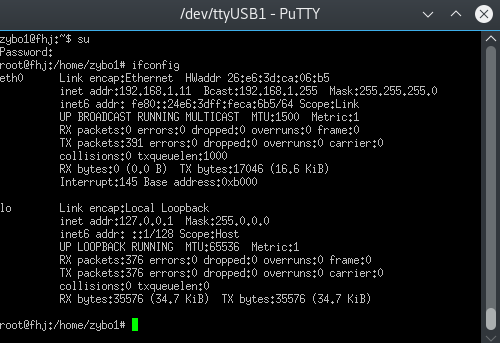
\includegraphics[scale=0.8]{Anexos/Anexo2/Infraestructura/ifconfigZybo.png}
	\caption{Interfaces de red en la tarjeta Zybo}
	\label{Interfaces de red en la tarjeta Zybo}
\end{figure}

Para asociar una dirección IP al nombre de cada dispositivo, tendremos que rellenar el fichero \texttt{/etc/hosts} de todos los dispositivos con las direcciones IP y el nombre de los dispositivos conectados a la red. Este archivo será idéntico en todos los dispositivos para garantizar una consistente agenda de direcciones.

Este proyecto ha sido diseñado para que se puedan usar tantas tarjetas como se requiera o como permitan las capacidades físicas de la red ya que solo habrá que ajustar el fichero\texttt{/etc/hosts} para añadir más nodos en caso de que sea necesario.

Todo el proceso de asignación de IP's para la creación de la infraestructura de red, lo podemos ver en el anexo \hyperlink{CreacionInfraestructura}{Creación de una infraestructura de red de tarjetas Zybo}.

A la hora de hacer las pruebas del proyecto, hemos usado solo tres nodos cifradores/descifradores ya que es suficiente como para comprobar el correcto funcionamiento del mismo.

\textcolor{red}{Añadir un dibujo de la red con sus plaquitas, el switch, los cables y el ordenador de la forma más ordenada que pueda.}

\subsection{Software}
%Aquí explicamos lo citado en el apartado de análisis.
El proceso de comunicación se inicia en el ordenador monitor cuando éste envía un fichero a la primera tarjeta Zybo. Cuando ésta lo recibe, descifra el contenido, introduce los cambios necesarios, cifra el fichero y lo envía a la siguiente tarjeta.

Dicho proceso se lleva a cabo de la misma forma entre todas las tarjetas hasta que se llega a la última de éstas\footnote{Esto se puede ver en el archivo \texttt{/etc/hosts}, donde están almacenadas todas las direcciones IP de los dispositivos.}, la cual envía el archivo nuevamente al ordenador monitor.

Toda esta comunicación se realiza gracias a la función de varios scripts programados en bash, por lo que tanto las tarjetas con Linux, como el ordenador monitor, son capaces de ejecutarlos.

Dichos scripts estarán automatizados mediante crontab\footnote{Crontab es un administrador regular de procesos en segundo plano que ejecuta procesos o guiones a intervalos regulares.}. Los podemos encontrar en el \hyperlink{Scripts}{Apéndice B} y se corresponden con la siguiente secuencia:
\begin{enumerate}
	\item Recepción del fichero: Proceso llevado a cabo por el script \hyperlink{ScriptRecibiendo}{\texttt{Recibiendo.sh}}. Gracias al comando \texttt{stat} de Linux, podemos comprobar el estado del directorio de forma cíclica para poder detectar cualquier cambio (como la recepción de un fichero) en cuanto se produzca.
	\item Descifrado, adición de datos y cifrado del fichero: Proceso llevado a cabo por el script \hyperlink{ScriptCristian}{\texttt{Cristian.sh}}. \textcolor{red}{Esto cambiará de nombre una vez que tenga lo de Gabri implementado.}
	\item Envío del fichero: Proceso llevado a cabo por el script \hyperlink{ScriptEnviando}{\texttt{Enviando.sh}}. Gracias al protocolo SSH y a la herramienta \texttt{sshpass}\footnote{Esta herramienta es necesaria para poder funcionar automáticamente sin tener que aceptar manualmente la conexión con el servidor.} de Linux, podremos enviar de forma automática el fichero modificado al siguiente nodo de la red.
\end{enumerate}

En caso de que se quieran vaciar los directorios de trabajo, siempre se podrá lanzar de forma manual el script \hyperlink{ScriptBorrar}{Borrar.sh}.